%% ============================================================
%%  SECCIÓN 6 — Procedimiento Experimental
%% ============================================================

\section{Procedimiento Experimental}
\label{sec:procedimiento}

A continuación se detalla el protocolo experimental ejecutado en el laboratorio para la caracterización de los tres componentes resistivos, estructurado de manera secuencial y cronológica.

\subsection{Montaje y Verificación del Circuito Potenciométrico}
\begin{enumerate}
    \item \textbf{Inspección y reconocimiento de componentes:} Se identificaron los terminales de la caja de elementos bajo prueba: la lámpara incandescente de filamento (\textbf{E1}), la resistencia de carbón de valor nominal \qty{100}{\ohm} (\textbf{E2}) y el diodo semiconductor de silicio (\textbf{E3}).
    \item \textbf{Configuración del divisor de tensión:} Se conectaron los dos extremos fijos del reóstato de laboratorio a los bornes de salida de la fuente de alimentación de corriente continua (DC).
    \item \textbf{Ajuste del potencial de entrada:} Con la carga desconectada, se encendió la fuente y se reguló su tensión de salida fija en \qty{7,50 \pm 0,05}{\volt}.
    \item \textbf{Calibración de cero:} Se desplazó el cursor móvil del reóstato hacia el extremo conectado al polo negativo (tierra común) y se verificó con el voltímetro que la diferencia de potencial entre el cursor y dicho polo fuera estrictamente de \qty{0,00}{\volt}.
    \item \textbf{Inserción de la instrumentación de medida:} Se derivó la línea del cursor móvil pasando en serie a través del amperímetro digital hacia el borne positivo ($a$) de la carga, y desde el borne negativo ($b$) se retornó a la línea común del potenciómetro. El voltímetro digital se conectó en derivación directa (paralelo) entre los nodos $a$ y $b$ (Figura~\ref{fig:esquema_circuito_teorico}).
\end{enumerate}

\begin{figure}[H]
    \centering
    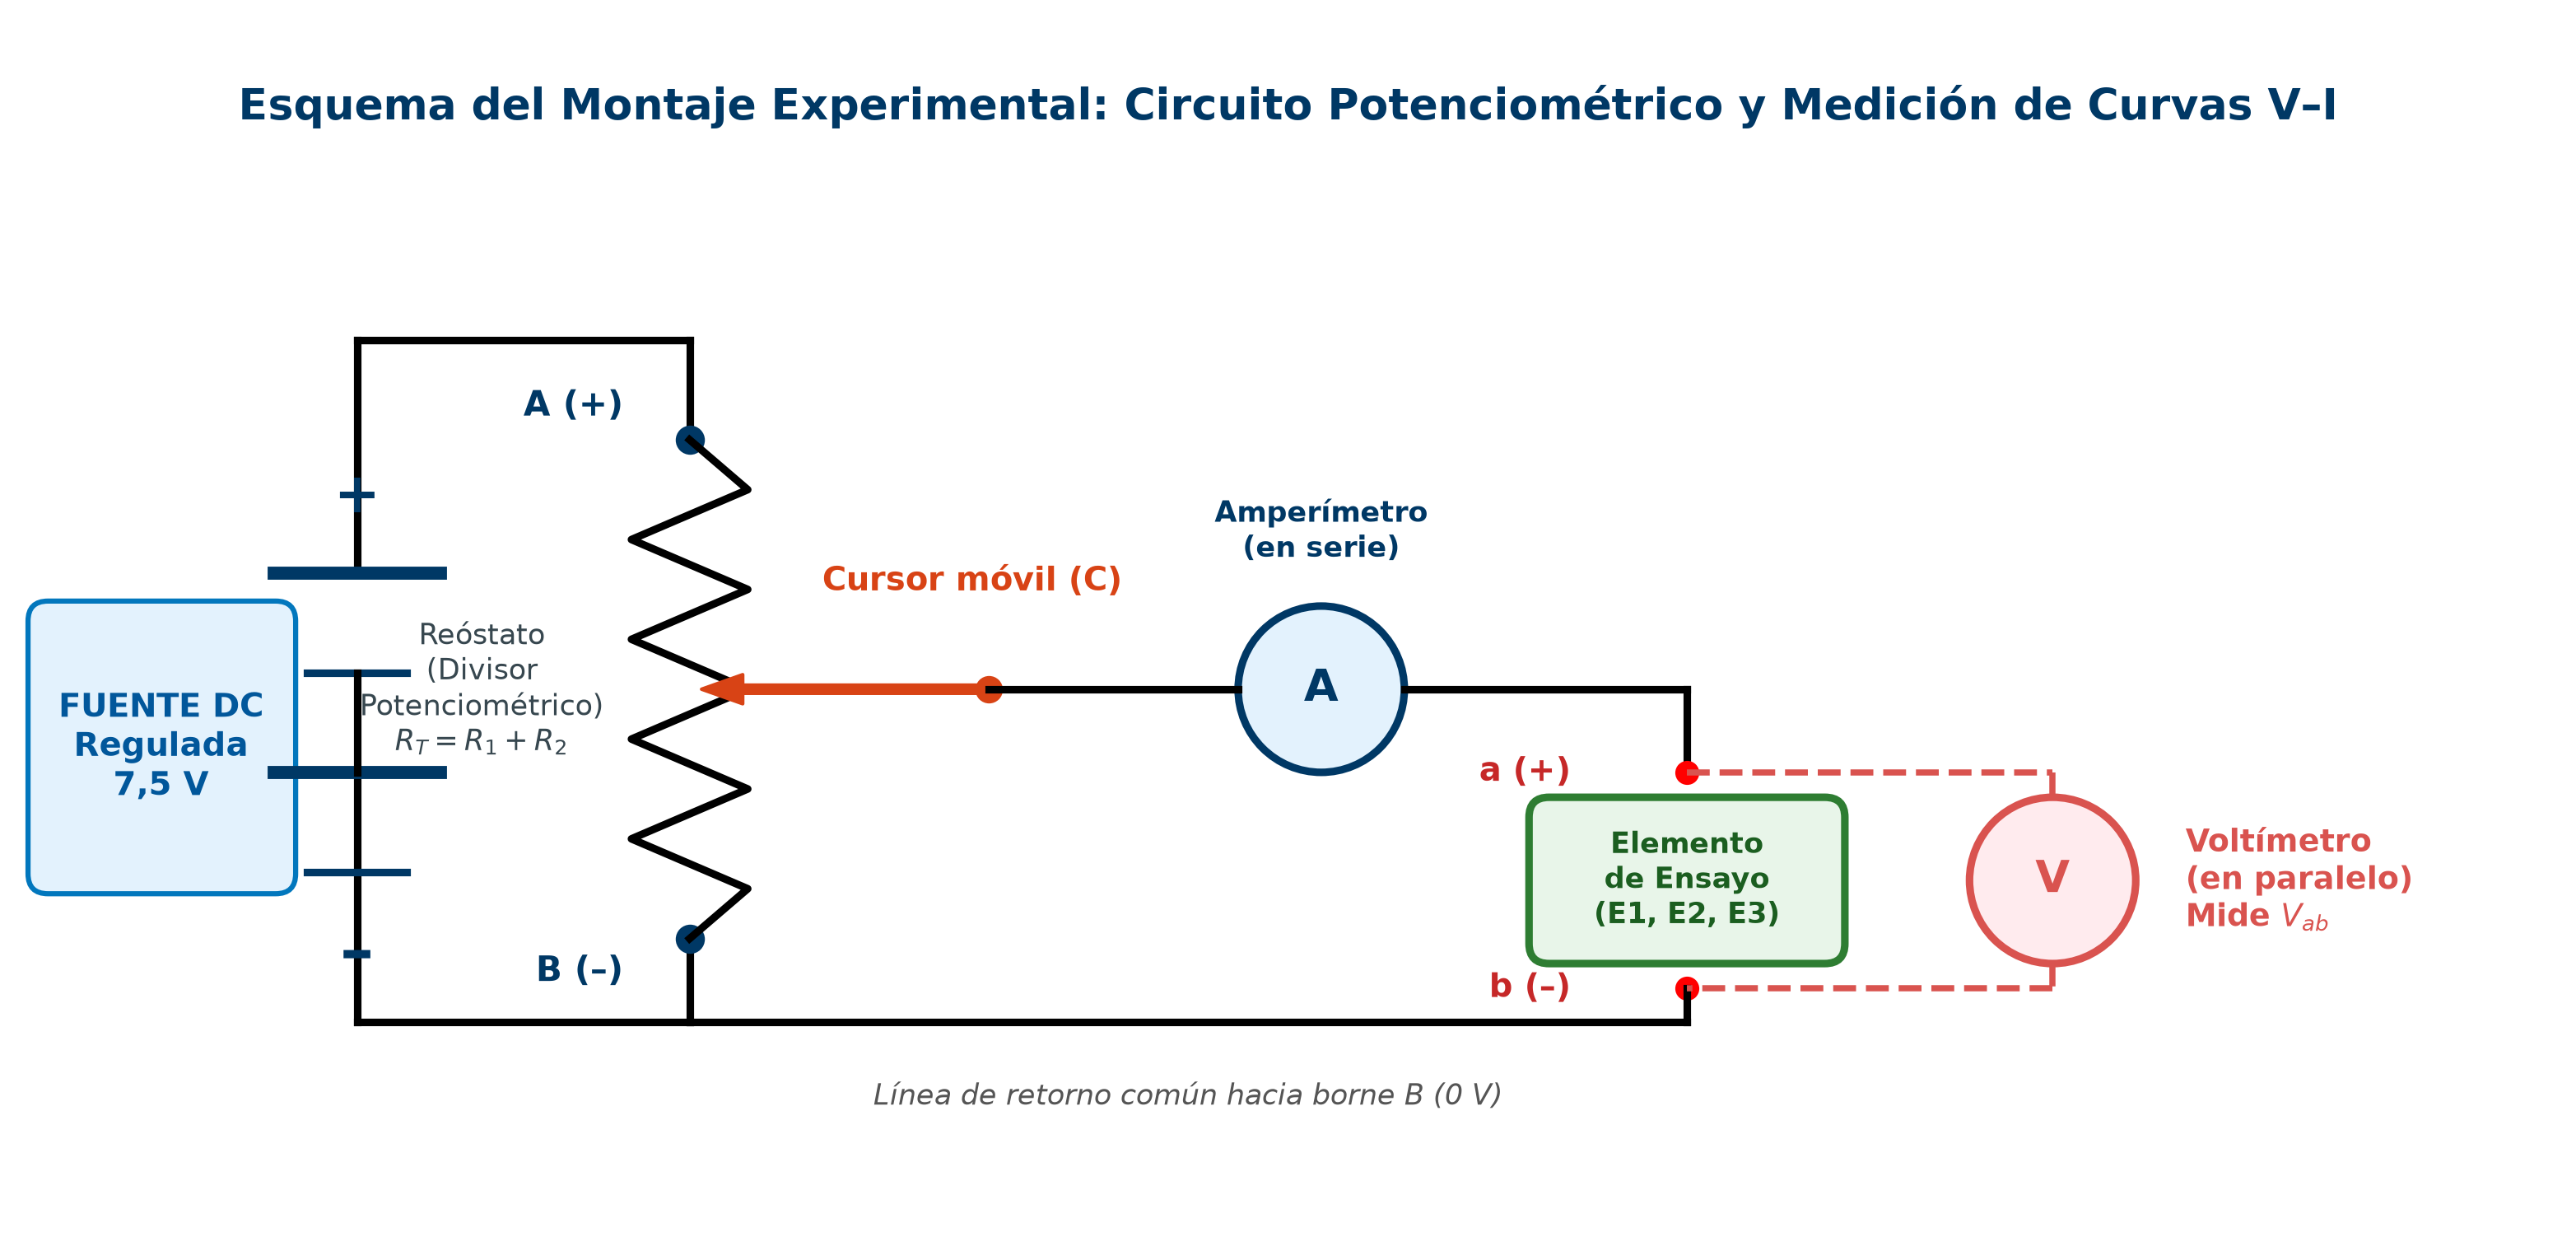
\includegraphics[width=0.75\linewidth]{fig_circuito_potenciometro}
    \caption{Esquema circuital del montaje potenciométrico con reóstato divisor de tensión, voltímetro en derivación y amperímetro en serie con el elemento bajo prueba.}
    \label{fig:esquema_circuito_teorico}
\end{figure}

\subsection{Parte A --- Medición en la Lámpara Incandescente (Elemento E1)}
\begin{enumerate}
    \setcounter{enumi}{5}
    \item Se conectaron los bornes de prueba $a$ y $b$ a la lámpara incandescente de tungsteno (\textbf{E1}).
    \item Partiendo del cursor en la posición de potencial nulo ($V = \qty{0,00}{\volt}$, $I = \qty{0,000}{\ampere}$), se desplazó suavemente el contacto móvil del reóstato hasta que el voltímetro registró una diferencia de potencial de aproximadamente \qty{1,00}{\volt}.
    \item Se registró simultáneamente la intensidad de corriente correspondiente en el amperímetro digital.
    \item Se repitió el procedimiento incrementando la diferencia de potencial en pasos nominales sucesivos de aproximadamente \qty{1}{\volt} (\qty{2,02}{\volt}, \qty{3,04}{\volt}, \qty{4,01}{\volt}, \qty{5,01}{\volt} y \qty{6,01}{\volt}), alcanzando una deflexión máxima del reóstato en \qty{6,43}{\volt}. Se observó cualitativamente la transición desde el filamento apagado hasta la emisión de luz visible intensa a partir de \qty{3}{\volt}.
\end{enumerate}

\subsection{Parte B --- Medición en la Resistencia de Carbón (Elemento E2)}
\begin{enumerate}
    \setcounter{enumi}{9}
    \item Se desconectó la lámpara y se conectaron los terminales $a$ y $b$ a la resistencia de composición de carbón de \qty{100}{\ohm} (\textbf{E2}).
    \item Se retornó el cursor del reóstato a su posición inicial verificando corriente nula a potencial cero.
    \item Se desplazó el cursor para fijar tensiones sucesivas en pasos regulares: \qty{1,00}{\volt}, \qty{2,00}{\volt}, \qty{3,05}{\volt}, \qty{4,03}{\volt}, \qty{5,00}{\volt}, \qty{6,02}{\volt} y el límite superior alcanzado de \qty{6,49}{\volt}.
    \item En cada escalón se registró la corriente en el amperímetro digital, constatando la estabilidad térmica y la ausencia de derivas temporales en la lectura.
\end{enumerate}

\subsection{Parte C --- Medición en el Diodo Semiconductor de Silicio (Elemento E3)}
\begin{enumerate}
    \setcounter{enumi}{13}
    \item Se conectaron los terminales $a$ y $b$ al diodo semiconductor (\textbf{E3}) en configuración de polarización directa (ánodo conectado al potencial positivo del cursor móvil a través del amperímetro y cátodo al terminal común negativo).
    \item Se verificó que para tensiones inferiores a \qty{0,50}{\volt} la corriente registrada fuera indistinguible de cero ($I < \qty{0,001}{\ampere}$).
    \item Al aproximarse a la región del codo de conducción ($\approx \qty{0,60}{\volt}$), se efectuó un ajuste fino y milimétrico del cursor del reóstato para muestrear detalladamente la curva en la zona de alta sensibilidad: \qty{0,61}{\volt}, \qty{0,69}{\volt}, \qty{0,70}{\volt}, \qty{0,71}{\volt}, \qty{0,72}{\volt}, \qty{0,73}{\volt} y \qty{0,75}{\volt}.
    \item \textbf{Control estricto de seguridad térmica:} Se monitoreó en todo momento el amperímetro para garantizar que la corriente no superara bajo ninguna circunstancia el umbral crítico de seguridad de \qty{0,900}{\ampere}, deteniendo la toma de datos en \qty{0,783}{\ampere} para evitar el embalamiento térmico y la destrucción de la juntura $p$-$n$.
\end{enumerate}

\subsection{Parte D --- Elemento Nicrón}
\begin{enumerate}
    \setcounter{enumi}{17}
    \item La guía original del laboratorio contemplaba una cuarta experiencia con un conductor resistivo de nicrón (níquel-cromo). Dicho elemento fue formalmente omitido en la sesión experimental por indicación del docente de mesa debido a indisponibilidad de la muestra patronada en el módulo de trabajo.
\end{enumerate}